\documentclass{beamer}

\usepackage{graphicx,multicol}
\usepackage{beamerouterthememiniframes, beamercolorthemeann,srcltx,hyperref}
\usepackage{listings}

\setbeamercolor{normal text}{fg=black!70}
\setbeamertemplate{navigation symbols}{}%geen navigatie
\setbeamertemplate{blocks}[rounded][shadow=true]
\setbeamertemplate{footline}{%
\hspace*{-0.5cm} \raisebox{5pt}{\makebox[\paperwidth]{\hfill\makebox[10pt]{\scriptsize\insertframenumber}}}}
 
\setbeamertemplate{caption}{\raggedright\insertcaption\par}

\title{Meta-tracing JIT compilation}
\author{Maarten Vandercammen}
\date{}

\lstset{
  language=Scheme
}

\begin{document}

\begin{frame}[plain]

\includegraphics[width=0.4\paperwidth]{VUB_logo.jpg}
\vspace{2cm}
\titlepage
\end{frame}


\section{Introduction}

\begin{frame}{Some terminology}

\begin{columns}[c]
    \column{.45\textwidth}
        \begin{center}
       	 	\begin{figure}
            	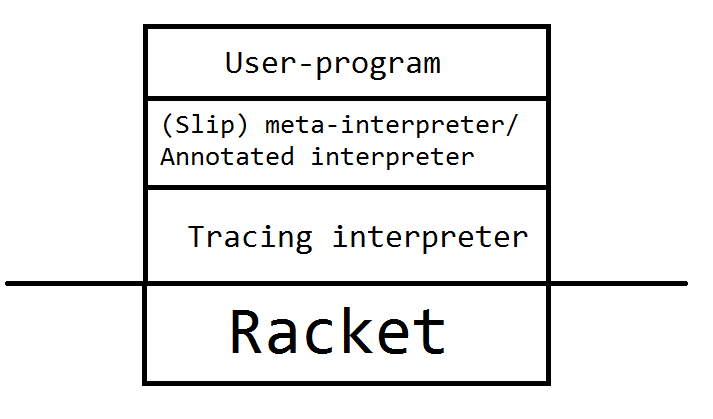
\includegraphics[scale = 0.32]{Terminology_1.png}
            	\caption{Regular meta-tracing}
        	\end{figure}
        \end{center}
    \pause
    \column{.45\textwidth}
        \begin{center}
       	 	\begin{figure}
            	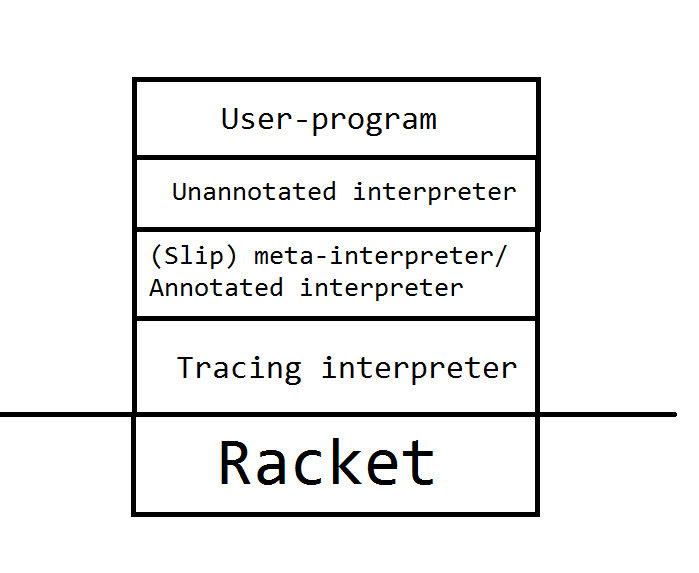
\includegraphics[scale = 0.32]{Terminology_2.png}
            	\caption{Nested meta-tracing}
        	\end{figure}
        \end{center}
\end{columns}

\end{frame}

\section{Regular interpretation}

\begin{frame}
\centering
\Huge{Regular interpretation}
\end{frame}

\begin{frame}[fragile]{CK-based register machine}

\begin{lstlisting}[basicstyle = \scriptsize\ttfamily, escapechar = £]

(define £\scriptsize$\rho$£ #f) ; env
  
(define £\scriptsize$\sigma$£ #f) ; store
  
(define £\scriptsize$\theta$£ #f) ; non-kont stack
  
(define v #f) ; general-purpose register

(struct ev (e £\small$\kappa$£) #:transparent)
  
(struct ko (£\small$\phi$£ £\small$\kappa$£) #:transparent)
\end{lstlisting}

\end{frame}

\begin{frame}[fragile]{Register manipulation}

\begin{center}
\begin{tabular}{c}
\begin{lstlisting}[basicstyle = \scriptsize\ttfamily, escapechar = £]
(save-val)
(restore-val)
(save-vals i)
(restore-vals i)
(save-all-vals)

(save-env)
(restore-env)
(set-env £\scriptsize$\rho$£*)

(alloc-var x)
(set-var x)
(lookup-var x)

(create-closure x es)
(literal-value e)
(quote-value e)
(apply-native i)

(push-continuation £\scriptsize$\phi$£)
(pop-continuation)
\end{lstlisting}
\end{tabular}
\end{center}

\end{frame}

\begin{frame}[fragile]{Step}

step = manipulate registers + return new CK state

\begin{lstlisting}[basicstyle = \scriptsize\ttfamily, escapechar = £]
; one evaluation step
(define new-state (step state)) 

(define (step state)
  (match state
    ((ev `(and ,e . ,es) £\scriptsize$\kappa$£)
     (execute/trace `(push-continuation ,(andk es)))
     (ev e (cons (andk es) £\scriptsize$\kappa$£)))
    ((ev (? symbol? x) (cons £\scriptsize$\phi$£ £\scriptsize$\kappa$£))
     (execute/trace `(lookup-var £'£,x) ; manipulate registers
                    `(pop-continuation))
     (ko £\scriptsize$\phi$£ £\scriptsize$\kappa$£)) ; return new state
     ...)
\end{lstlisting}

\end{frame}

\begin{frame}[fragile]{Step*}

\begin{lstlisting}[basicstyle = \small\ttfamily, escapechar = £]
; complete evaluation
(define result (step* state))

(define (step* state)
  (match state
    ((ko (haltk) _) ; evaluation finished
     v)
    (_
     (let ((new-state (step state)))
       (step* new-state)))))
\end{lstlisting}

\end{frame}

\begin{frame}[fragile]{Closures}

\begin{lstlisting}[basicstyle = \small\ttfamily, escapechar = £]
  (struct clo (£\small$\lambda$£ £\small$\rho$£) #:transparent)
  (struct lam (x es) #:transparent)
  
  (create-closure x es)
  
  (clo-equal? clo1 clo2)
\end{lstlisting}

\end{frame}

\section{Tracing}

\begin{frame}
\centering
\Huge{Tracing}
\end{frame}

\begin{frame}[fragile]{Annotations}

\begin{lstlisting}[basicstyle = \small\ttfamily, escapechar = £]
  (can-start-loop label debug-info)
  
  (can-close-loop label)
\end{lstlisting}

\end{frame}

\begin{frame}[fragile]{Annotations}

\begin{lstlisting}[basicstyle = \footnotesize\ttfamily, escapechar = £]
  (define (close parameters expressions closure-name)
      (define lexical-environment environment)
      (define (closure . arguments)
        (define dynamic-environment environment)
        ; function call starts here
        (can-start-loop expressions closure-name)
        (set! environment lexical-environment)
        (bind-parameters parameters arguments)
        (let* ((value (evaluate-sequence expressions)))
          (set! environment dynamic-environment)
          ; function call ends here
          (can-close-loop expressions)
          value))
      closure)
\end{lstlisting}

\end{frame}

\begin{frame}[fragile]{Handling annotations}

\begin{lstlisting}[basicstyle = \scriptsize\ttfamily, escapechar = £]
(define (step* state)
    (match state
      ((ko (haltk) _)
       v)
      ; evaluate annotations in step* instead of step
      ; annotations might not lead to recursive call to step*
      ((ko (can-close-loopk) (cons £\small$\phi$£ £\small$\kappa$£))
       (handle-can-close-loop-annotation v (ko £\small$\phi$£ £\small$\kappa$£)))
      ((ko (can-start-loopk £'£() debug-info) (cons £\small$\phi$£ £\small$\kappa$£))
       (handle-can-start-loop-annotation v debug-info (ko £\small$\phi$£ £\small$\kappa$£)))
      (_
       (let ((new-state (step state)))
         (step* new-state)))))
\end{lstlisting}

\end{frame}

\begin{frame}{Overview}

\centering
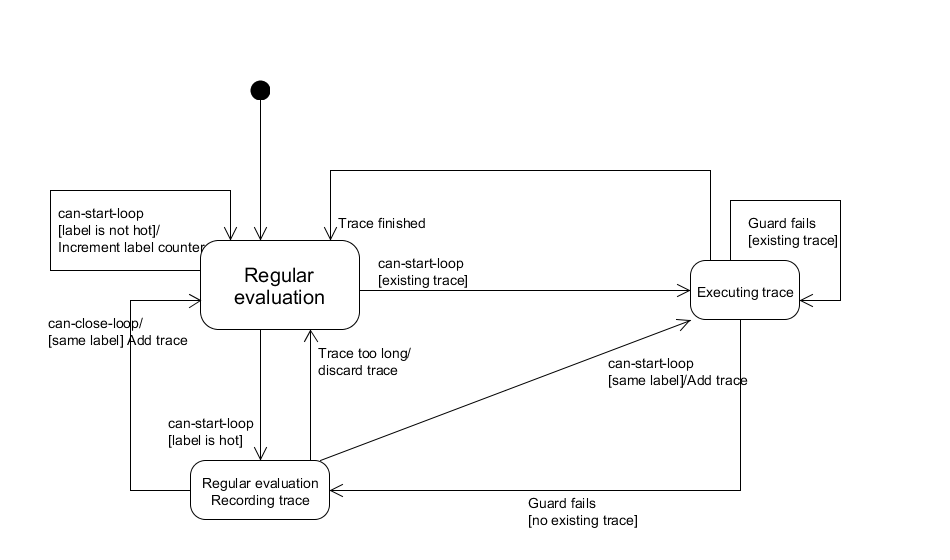
\includegraphics[scale=0.4]{high_level_state_diagram_no_merging.png} 

\end{frame}

\begin{frame}[fragile]{Guards}
\begin{lstlisting}[basicstyle = \small\ttfamily, escapechar = £]
(define (loop n)
  (display n) (newline)
  (if (< n 0)
      (display "Stopped!")
      (loop (- n 1))))
\end{lstlisting}
\end{frame}

\begin{frame}[fragile]{Guards}

\begin{lstlisting}[basicstyle = \small\ttfamily, escapechar = £]
(if bool a b) -> guard-false/guard-true
(cond ...) -> guard-false/guard-true
(f ...) -> guard-same-closure
(apply f (list ...)) -> guard-same-nr-of-args

(define (guard-true ...)
  (unless v
          ; do something
          ))
\end{lstlisting}

\end{frame}

\begin{frame}[fragile]{Guards}

Guards identified with id's

\begin{lstlisting}[basicstyle = \scriptsize\ttfamily, escapechar = £]
(define (step state)
  (match state
    ((ko (ifk e1 e2) £\small$\kappa$£)
       (execute/trace `(restore-env))
       (let ((new-guard-id (inc-guard-id!)))
         (if v
             (begin (execute/trace `(guard-true ,new-guard-id)) 
                    (ev e1 £\small$\kappa$£))
             (begin (execute/trace `(guard-false ,new-guard-id)) 
                    (ev (car e2) £\small$\kappa$£)))))
\end{lstlisting}

\end{frame}

\begin{frame}[fragile]{Bookkeeping}

\begin{lstlisting}[basicstyle = \scriptsize\ttfamily, escapechar = £]
(struct tracer-context (is-tracing?
                        trace-key
                        times-label-encountered-while-tracing
                        current-trace-length
                        labels-encountered
                        trace-nodes
                        trace-nodes-dictionary
                        labels-executing
                        closing-function
                        merges-cf-function
                        guards-dictionary) #:transparent #:mutable)
                        
(define GLOBAL_TRACER_CONTEXT (new-tracer-context))
\end{lstlisting}

\end{frame}

\begin{frame}{Two traces}

Label traces and guard traces

\centering
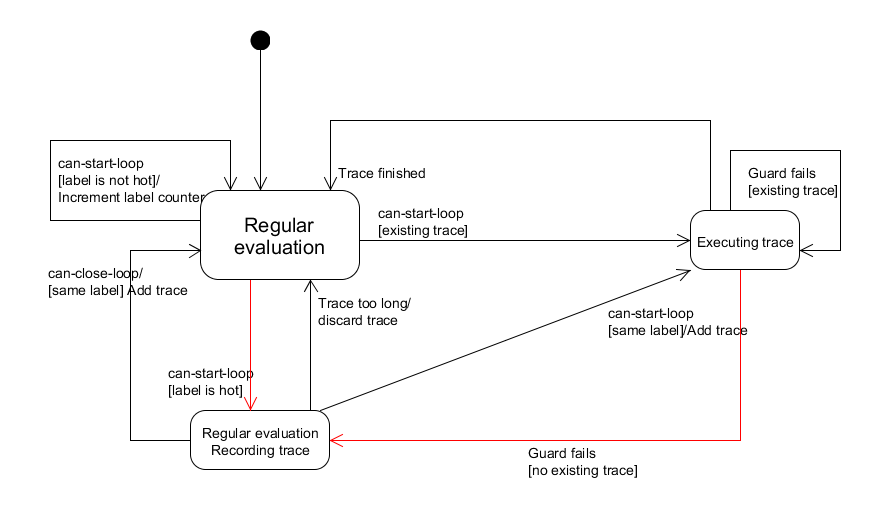
\includegraphics[scale=0.3]{high_level_state_diagram_two_traces.png}

\end{frame}

\begin{frame}[fragile]{(can-start-loop)}
\begin{lstlisting}[basicstyle = \tiny\ttfamily, escapechar = £]
  (define (handle-can-start-loop-annotation label debug-info state)
    ; Continue regular interpretation with the given state.
    (define (continue-with-state)
      (execute/trace `(pop-continuation))
      (step* state))
    ; Trace hot?
    (define (can-start-tracing-label?)
      (>= (get-times-label-encountered label) TRACING_THRESHOLD))
    (cond ((is-tracing-label? label)
           (stop-tracing! #t)
      	   (let ((new-state (execute-label-trace-with-label label)))
        	  (step* new-state)))
          ((label-trace-exists? label)
           ; Execute trace
           (let* ((label-trace (get-label-trace label))
                  ((new-state (execute-label-trace-with-label label)))
             (step* new-state)))
          ((and (not (is-tracing?)) (can-start-tracing-label?))
           (start-tracing-label! label debug-info)
           (continue-with-state))
          ; Increase £'£hotness£'£ counter of label
          (else
           (inc-times-label-encountered! label)
           (continue-with-state))))
\end{lstlisting}
\end{frame}

\begin{frame}[fragile]{Starting tracing}
\begin{lstlisting}[basicstyle = \scriptsize\ttfamily, escapechar = £]
; Starting tracing = doing some bookkeeping!
(define (start-tracing-guard! guard-id old-trace-key)
    (clear-trace!)
    (set-tracer-context-is-tracing?! GLOBAL_TRACER_CONTEXT #t)
    (set-tracer-context-trace-key! GLOBAL_TRACER_CONTEXT (make-guard-trace-key (trace-key-label old-trace-key)
                                                                               (get-parent-label-trace-id old-trace-key))))
  
  (define (start-tracing-label! label debug-info)
    (clear-trace!)
    (set-tracer-context-is-tracing?! GLOBAL_TRACER_CONTEXT #t)
    (set-tracer-context-trace-key! GLOBAL_TRACER_CONTEXT (make-label-trace-key label debug-info)))
\end{lstlisting}
\end{frame}

\begin{frame}[fragile]{Starting tracing}

\begin{lstlisting}[basicstyle = \small\ttfamily, escapechar = £]
; Keep track of what you£'£re tracing
(struct trace-key (label id) #:transparent)

; Store id of parent label that caused guard failure
(struct guard-trace-key trace-key (parent-label-trace-id) #:transparent)

(struct label-trace-key trace-key (debug-info) #:transparent)
\end{lstlisting}

\end{frame}

\begin{frame}[fragile]{Recording operations}

\begin{lstlisting}[basicstyle = \small\ttfamily, escapechar = £]
(define £\small$\tau$£ £'£())

(define (append-trace! ms)
  (let ((new-instructions-length (length ms)))
    (set! £\small$\tau$£ (append (reverse ms) £\small$\tau$£))
    (add-trace-length! new-instructions-length))))

(define (execute/trace . ms)
  (when (is-tracing?)
    (append-trace! ms))
  (eval-instructions ms))
\end{lstlisting}

\end{frame}

\begin{frame}[fragile]{Stopping tracing}

\centering
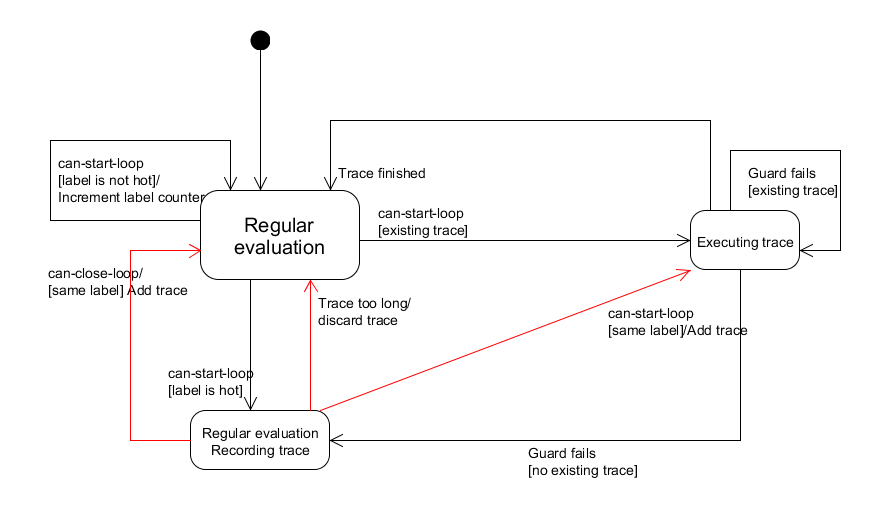
\includegraphics[scale=0.3]{high_level_state_diagram_stopping_tracing.png}

\end{frame}

\begin{frame}[fragile]{Trace too long}

\begin{lstlisting}[basicstyle = \footnotesize\ttfamily, escapechar = £]
; Final version
(define (append-trace! ms)
  (let ((new-instructions-length (length ms)))
    (set! £\footnotesize$\tau$£ (append (reverse ms) £\footnotesize$\tau$£))
    (add-trace-length! new-instructions-length)
    (when (max-trace-length-reached?)
      (handle-max-trace-length-reached))))
      
(define (handle-max-trace-length-reached)
  ; Stop tracing and discard the trace
  (stop-tracing-abnormal!))
\end{lstlisting}

\end{frame}

\begin{frame}[fragile]{Looping vs non-looping}

\begin{columns}[c]
    \column{0.35 \textwidth}
\begin{lstlisting}[basicstyle = \footnotesize\ttfamily, escapechar = £]
; No recursion -> no looping
(define (f x)
  (+ x 1))
\end{lstlisting}
Ends with (can-close-loop)
\pause

\column{0.4 \textwidth}
\begin{lstlisting}[basicstyle = \footnotesize\ttfamily, escapechar = £]
; Recursion -> looping
(define (f x)
  (f x))
\end{lstlisting}
Ends with (can-start-loop label debug-info)
\end{columns}
\end{frame}

\begin{frame}[fragile]{Looping vs non-looping}
\begin{lstlisting}[basicstyle = \footnotesize\ttfamily, escapechar = £]
(define (handle-can-close-loop-annotation label state)
    (when (is-tracing-label? label)
      ; #f = label does not loop
      (stop-tracing! #f))
    (execute/trace `(pop-continuation))
    (step* state))
    
(define (handle-can-start-loop-annotation label debug-info state)
    (cond ((is-tracing-label? label)
           ; #t = label does loop
           (stop-tracing! #t)
           (let ((new-state (execute-label-trace-with-label label)))
             (step* new-state))))
\end{lstlisting}
\end{frame}

\begin{frame}[fragile]{Looping vs non-looping}

Labels:
\begin{columns}[c]
    \column{0.35 \textwidth}
\begin{lstlisting}[basicstyle = \footnotesize\ttfamily, escapechar = £]
; Recursion -> looping
(letrec ((loop (lambda ()
    ; trace instructions
    (loop))))
  (loop))
\end{lstlisting}
\pause

\column{0.4 \textwidth}
\begin{lstlisting}[basicstyle = \footnotesize\ttfamily, escapechar = £]
; No recursion -> no looping
(letrec ((non-loop (lambda ()
    ; trace instructions
    )))
  (non-loop))
\end{lstlisting}
\end{columns}

\end{frame}

\begin{frame}[fragile]{Looping vs non-looping}
Guards:
\begin{lstlisting}[basicstyle = \scriptsize\ttfamily, escapechar = £]
(define (f)
  (if (= (random 2) 0)
      (begin (display 0)
             (f))
      (begin (display 1)
             (f))))
\end{lstlisting}
\end{frame}

\begin{frame}[fragile]{Looping vs non-looping}

Guards:
\begin{columns}[c]
    \column{0.4 \textwidth}
\begin{lstlisting}[basicstyle = \scriptsize\ttfamily, escapechar = £]
; Recursion -> looping
(letrec ((non-loop (lambda ()
    ; trace instructions
    )))
  (non-loop)
  (execute-label-trace-with-id parent-label-trace-id))
\end{lstlisting}
\pause

\column{0.4 \textwidth}
\begin{lstlisting}[basicstyle = \scriptsize\ttfamily, escapechar = £]
; Recursion -> looping
(letrec ((non-loop (lambda ()
    ; trace instructions
    )))
  (non-loop))
\end{lstlisting}
\end{columns}

\end{frame}

\begin{frame}[fragile]{Stop tracing normally}

Scheme-style state pattern: \\
first-class functions

\begin{lstlisting}[basicstyle = \scriptsize\ttfamily, escapechar = £]
(define (start-tracing-guard! guard-id old-trace-key)
  ...
  (set-tracer-context-closing-function! GLOBAL_TRACER_CONTEXT (make-stop-tracing-guard-function guard-id))
  ...)
  
(define (start-tracing-label! label debug-info)
  ...
  (set-tracer-context-closing-function! GLOBAL_TRACER_CONTEXT (make-stop-tracing-label-function))
  ...)
\end{lstlisting}

\end{frame}

\begin{frame}[fragile]{Stop tracing normally}

Closing functions: transform trace correctly and add trace

\begin{lstlisting}[basicstyle = \scriptsize\ttfamily, escapechar = £]
(define (stop-tracing-label! trace looping?)
  (let* ((trace-key (tracer-context-trace-key GLOBAL_TRACER_CONTEXT))
         (transformed-trace (transform-and-optimize-trace trace (make-transform-label-trace-function looping?))))
    (add-label-trace! trace-key transformed-trace looping?)))
\end{lstlisting}

\pause

\begin{lstlisting}[basicstyle = \scriptsize\ttfamily, escapechar = £]
(define (make-transform-label-trace-function looping?)
  (if looping?
      transform-label-trace-looping
      transform-trace-non-looping))
\end{lstlisting}
\end{frame}

\begin{frame}[fragile]{Transforming traces}

\begin{lstlisting}[basicstyle = \footnotesize\ttfamily, escapechar = £]
(define (transform-trace-non-looping trace)
  `(letrec ((non-loop ,(append £'£(lambda ()) trace)))
     (non-loop)))
\end{lstlisting}

\begin{lstlisting}[basicstyle = \footnotesize\ttfamily, escapechar = £]
(define (transform-label-trace-looping trace)
  `(letrec ((loop ,(append £'£(lambda ()) trace £'£((loop)))))
     (loop)))
\end{lstlisting}

\end{frame}

\begin{frame}[fragile]{Stop tracing normally}

\begin{lstlisting}[basicstyle = \scriptsize\ttfamily, escapechar = £]
(define (stop-tracing! looping?)
    (let ((stop-tracing-function (tracer-context-closing-function GLOBAL_TRACER_CONTEXT)))
      (stop-tracing-function (reverse £\footnotesize$\tau$£) looping?)
      (stop-tracing-normal!)))
  
  (define (stop-tracing-normal!)
    (stop-tracing-bookkeeping!))
      
(define (stop-tracing-bookkeeping!)
    (set-tracer-context-is-tracing?! GLOBAL_TRACER_CONTEXT #f)
    (set-tracer-context-trace-key! GLOBAL_TRACER_CONTEXT #f)
    (set-tracer-context-closing-function! GLOBAL_TRACER_CONTEXT #f)
    (clear-trace!))
\end{lstlisting}

\end{frame}

\begin{frame}[fragile]{Intermezzo}

Trace representation

\begin{lstlisting}[basicstyle = \scriptsize\ttfamily, escapechar = £]
(struct trace-node (trace-key
                    trace
                    (executions #:mutable)))
                    
(struct tracer-context (...
                        trace-nodes
                        trace-nodes-dictionary
                        guards-dictionary
                        ...)
\end{lstlisting}

\end{frame}

\begin{frame}[fragile]{Trace execution}

\centering
Trace execution = call eval on trace

\pause

\vspace{2cm}

Actually... for-each eval on trace operations

\end{frame}

\begin{frame}[fragile]{Trace execution}

\begin{lstlisting}[basicstyle = \tiny\ttfamily, escapechar = £]
(define (execute-guard-trace guard-id)
    (let* ((guard-trace (get-guard-trace guard-id))
           (trace (trace-node-trace guard-trace)))
      ; Benchmarking
      (add-execution! guard-trace)
      (execute/trace
               ; Actually execute the trace
        `(let* ((state (execute-trace £'£,trace))) 
           ; Don£'£t mind this!
           (bootstrap-to-evaluator state)))))
  
  (define (execute-label-trace-with-trace-node label-trace-node)
    (let ((trace (trace-node-trace label-trace-node)))
      ; Benchmarking
      (add-execution! label-trace-node)
      (execute/trace
        `(let ()
           (push-label-trace-executing! ,label-trace-node)
                ; Actually execute the trace
           (let ((state (execute-trace £'£,trace))) 
           (pop-label-trace-executing!)
           ; Don£'£t mind this!
           state)))))
\end{lstlisting}
\end{frame}
  
\begin{frame}[fragile]{Trace execution}
\begin{lstlisting}[basicstyle = \scriptsize\ttfamily, escapechar = £]
  (define (execute-label-trace-with-id label-trace-id)
         ; find trace
    (let ((label-trace-node (find (tracer-context-trace-nodes-dictionary GLOBAL_TRACER_CONTEXT) label-trace-id)))
      ; execute trace
      (execute-label-trace-with-trace-node label-trace-node)))
  
  (define (execute-label-trace-with-label label)
         ; find trace
    (let ((label-trace-node (get-label-trace label)))
      ; execute trace
      (execute-label-trace-with-trace-node label-trace-node)))
\end{lstlisting}

\end{frame}

\begin{frame}[fragile]{Trace execution}
Identify label trace being executed
\begin{lstlisting}[basicstyle = \footnotesize\ttfamily, escapechar = £]
(push-label-trace-executing! label-trace-node)
(pop-label-trace-executing!)
(top-label-trace-executing)

(struct tracer-context (...
                        labels-executing
                        ...)
                        
(define (guard-failed guard-id state)
  (cond ((not (is-tracing?))
         (let ((trace-key-executing (get-label-trace-executing-trace-key)))
           ...)))
\end{lstlisting}
\end{frame}

\begin{frame}[fragile]{Trace execution}
Why a stack? Trace jumping!
\begin{lstlisting}[basicstyle = \footnotesize\ttfamily, escapechar = £]
(define (f x)
  (+ x 10))
  
(define (loop)
  (f 1)
  ; other stuff
  (loop))
\end{lstlisting}
\end{frame}

\begin{frame}[fragile]{Stopping trace execution}
\centering
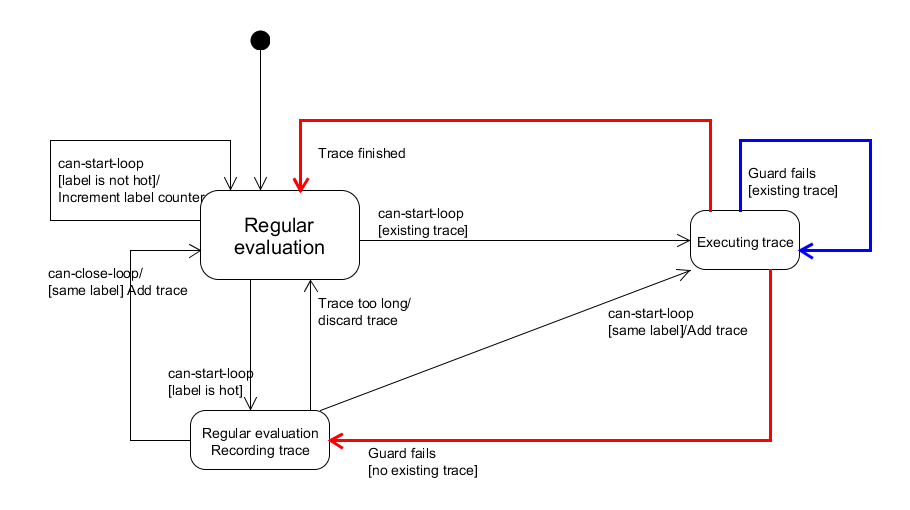
\includegraphics[scale=0.3]{high_level_state_diagram_stop_trace_execution.png}
\end{frame}

\begin{frame}[fragile]{Stopping trace execution}
Two problems:

\begin{itemize}
\item Stop trace execution
\item Continue with regular interpretation
\end{itemize}

\end{frame}

\begin{frame}[fragile]{Restart interpretation}
Bootstrap interpreter with CK state $\rightarrow$ \\
Reconstruct expected continuation

\pause

\vspace{1cm}

Operations on K invisible in trace $\rightarrow$ \\ K gets lost during trace execution

\pause

Use register for K

\pause

\vspace{0.5cm}

C? Later

\end{frame}

\begin{frame}[fragile]{$\tau$-$\kappa$}

\begin{lstlisting}[basicstyle = \scriptsize\ttfamily, escapechar = £]
(define £\footnotesize$\tau$£-£\scriptsize$\kappa$£ £'£()) ;continuation stack

(push-continuation £\scriptsize$\phi$£)
(pop-continuation)

(define (step state)
  (match state
    ((ev (? symbol? x) (cons £\scriptsize$\phi$£ £\scriptsize$\kappa$£))
     (execute/trace `(lookup-var £'£,x)
                    `(pop-continuation))
     (ko £\scriptsize$\phi$£ £\scriptsize$\kappa$£))
\end{lstlisting}

\end{frame}

\begin{frame}[fragile]{Restart interpretation}
\begin{lstlisting}[basicstyle = \scriptsize\ttfamily, escapechar = £]
(define (transform-trace-non-looping trace)
    `(letrec ((non-loop ,(append £'£(lambda ()) trace)))
       (non-loop)
            ; Use £\scriptsize{\color[rgb]{0.133,0.545,0.133}$\tau$}£-£\scriptsize{\color[rgb]{0.133,0.545,0.133}$\kappa$}£ to reconstruct state
       (let ((new-state (ko (car £\scriptsize$\tau$£-£\scriptsize$\kappa$£) (cdr £\scriptsize$\tau$£-£\scriptsize$\kappa$£))))
         (pop-continuation)
         new-state)))
\end{lstlisting}
\end{frame}

\begin{frame}[fragile]{Non-looping label-traces}
\begin{lstlisting}[basicstyle = \scriptsize\ttfamily, escapechar = £]
(define (handle-can-start-loop-annotation label debug-info state)
  (cond ((label-trace-exists? label)
         (let* ((label-trace (get-label-trace label))
                (new-state (execute-label-trace-with-label label)))
           (step* new-state))))
  
(define (execute-label-trace-with-trace-node label-trace-node)
  (let ((trace (trace-node-trace label-trace-node)))
    ; Benchmarking
    (add-execution! label-trace-node)
    (execute/trace
      `(let ()
         (push-label-trace-executing! ,label-trace-node)
              ; Actually execute the trace
         (let ((state (execute-trace £'£,trace)))
           (pop-label-trace-executing!)
           state)))))
\end{lstlisting}
\end{frame}

\begin{frame}[fragile]{Non-looping guard-traces}
\begin{lstlisting}[basicstyle = \scriptsize\ttfamily, escapechar = £]
(define (execute-guard-trace guard-id)
    (let* ((guard-trace (get-guard-trace guard-id))
           (trace (trace-node-trace guard-trace)))
      ; Benchmarking
      (add-execution! guard-trace)
      (execute/trace
        `(let ()
                 ; Actually execute the trace
           (let* ((state (execute-trace £'£,trace)))
             ; Actually incorrect...
             (bootstrap-to-evaluator state))))))
\end{lstlisting}
\end{frame}

\begin{frame}[fragile]{Looping traces}
Ending looping traces = only through guard-failure
\begin{lstlisting}[basicstyle = \tiny\ttfamily, escapechar = £]
 (define (guard-failed guard-id state)
    (cond ((guard-trace-exists? guard-id)
           (execute-guard-trace guard-id))
          ((not (is-tracing?))
           ; Start tracing guard
           ; Get label being executed!
           (let ((trace-key-executing (get-label-trace-executing-trace-key)))
             (start-tracing-guard! guard-id trace-key-executing)
             (bootstrap-to-evaluator state)))
          (else
           ; Already tracing something else:
           ; stop tracing that and start tracing this guard!
           (let ((trace-key-executing (get-label-trace-executing-trace-key)))
             (switch-to-trace-guard! guard-id trace-key-executing)
             (bootstrap-to-evaluator state)))))
\end{lstlisting}
\end{frame}

\begin{frame}[fragile]{State?}
Reconstruct C in CK?

\begin{lstlisting}[basicstyle = \scriptsize\ttfamily, escapechar = £]
(define (guard-true guard-id e)
  (unless v
    (guard-failed-with-ev guard-id e))))
      
(define (guard-failed-with-ev guard-id e)
  (guard-failed guard-id (ev e £\footnotesize$\tau$£-£\footnotesize$\kappa$£)))

(define (step state)
  (match state
   ((ko (ifk e1 e2) £\footnotesize$\kappa$£)
    ...
    (if v
        (begin (execute/trace 
                 `(guard-true ,new-guard-id £'£,e2))
               (ev e1 £\scriptsize$\kappa$£))
        ...))
\end{lstlisting}
\end{frame}

\begin{frame}[fragile]{Stopping trace execution}

\begin{lstlisting}[basicstyle = \small\ttfamily, escapechar = £]
(eval £'£((save-env)
       (lookup-var £'£x)
       ...
       (guard-true 123 ...)
       (apply-native £'£+ 3)
       ...))
\end{lstlisting}

\pause

Call/cc!

\end{frame}

\begin{frame}[fragile]{Call/cc}
\begin{lstlisting}[basicstyle = \scriptsize\ttfamily, escapechar = £]
(define GLOBAL_CONTINUATION #f)

(define (set-global-continuation! k)
  (set! GLOBAL_CONTINUATION k))
  
(define (call-global-continuation v)
  (GLOBAL_CONTINUATION v))
  
(define (run start-state)
  (apply step*
         (list (let ((state (call/cc
                              (lambda (k)
                                (set-global-continuation! k)
                                start-state))))
                 ; Start regular interpretation -> no trace executions
                 (flush-label-traces-executing!)
                 state))))
\end{lstlisting}
\end{frame}

\begin{frame}[fragile]{Call/cc}
\begin{lstlisting}[basicstyle = \tiny\ttfamily, escapechar = £]
(define (bootstrap-to-evaluator state)
  (call-global-continuation state))
  
(define (execute-guard-trace guard-id)
    (let* ((guard-trace (get-guard-trace guard-id))
           (trace (trace-node-trace guard-trace)))
      ; Benchmarking
      (add-execution! guard-trace)
      (execute/trace
        `(let ()
                 ; Actually execute the trace              
           (let* ((state (execute-trace £'£,trace)))
             ;Incorrect...
             (bootstrap-to-evaluator state))))))
  
(define (execute-label-trace-with-trace-node label-trace-node)
  (let ((trace (trace-node-trace label-trace-node)))
    ; Benchmarking
    (add-execution! label-trace-node)
    (execute/trace
      `(let ()
         (push-label-trace-executing! ,label-trace-node)
              ; Actually execute the trace
         (let ((state (execute-trace £'£,trace))) 
           (pop-label-trace-executing!)
           ; No bootstrapping!!!
           state)))))
\end{lstlisting}
\end{frame}

\begin{frame}[fragile]{Trace execution}
Why no bootstrapping? Trace jumping!
\begin{lstlisting}[basicstyle = \footnotesize\ttfamily, escapechar = £]
(define (f x)
  (+ x 10))
  
(define (loop)
  (f 1)
  ; other stuff
  (loop))
\end{lstlisting}
\end{frame}

\begin{frame}[fragile]{Trace execution}
And remember
\begin{lstlisting}[basicstyle = \footnotesize\ttfamily, escapechar = £]
(define (handle-can-start-loop-annotation label debug-info state)
  (cond ((label-trace-exists? label)
         (let* ((label-trace (get-label-trace label))
                ; Also safe without trace jumping
                (new-state (execute-label-trace-with-label label)))
           ; When evaluating non-looping trace no need for bootstrapping
           (step* new-state)))
\end{lstlisting}
\end{frame}

\begin{frame}[fragile]{Trace execution}
Why are guard-trace executions incorrect?
\begin{lstlisting}[basicstyle = \footnotesize\ttfamily, escapechar = £]
(define (f)
  (if (= (random 2) 0)
      (display 0)
      (display 1)))
  
(define (loop)
  (f)
  ; other stuff
  (loop))
\end{lstlisting}
\end{frame}

\begin{frame}[fragile]{Trace jumping}
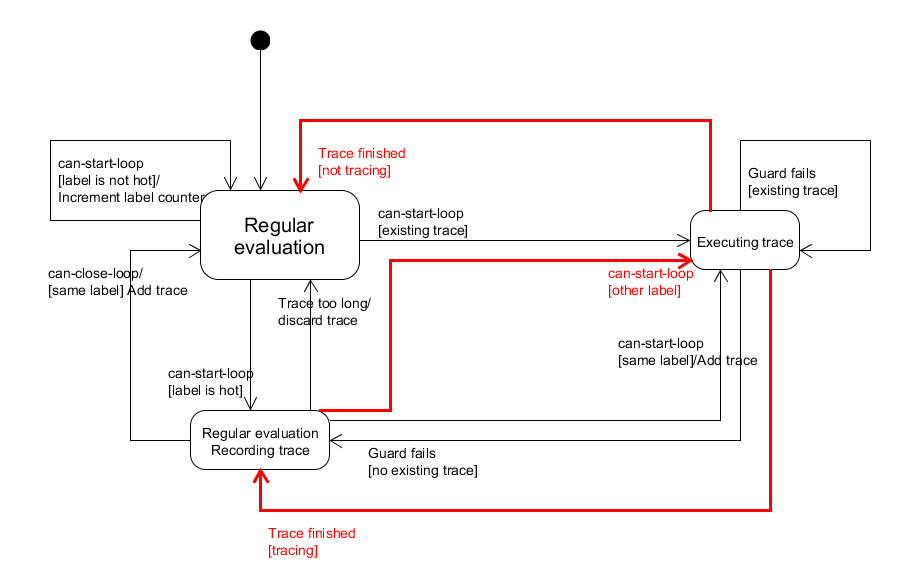
\includegraphics[scale=0.3]{stopping_trace_exec_while_tracing.png} 
\end{frame}

\begin{frame}[fragile]{Trace jumping}

Remember

\begin{lstlisting}[basicstyle = \tiny\ttfamily, escapechar = £]
(define (handle-can-start-loop-annotation label debug-info state)
  (cond ; Don£'£t check whether already tracing
        ((label-trace-exists? label)
         ; Execute trace
         (let* ((label-trace (get-label-trace label))
                ((new-state (execute-label-trace-with-label label)))
           ...))))
           
(define (execute-label-trace-with-trace-node label-trace-node)
  (let ((trace (trace-node-trace label-trace-node)))
    ; Benchmarking
    (add-execution! label-trace-node)
    ; Automatically traced
    (execute/trace
      `(let ()
         (push-label-trace-executing! ,label-trace-node)
              ; Actually execute the trace
         (let ((state (execute-trace £'£,trace))) 
           ...)))))
\end{lstlisting}
\end{frame}

\begin{frame}[fragile]{True vs false loops}
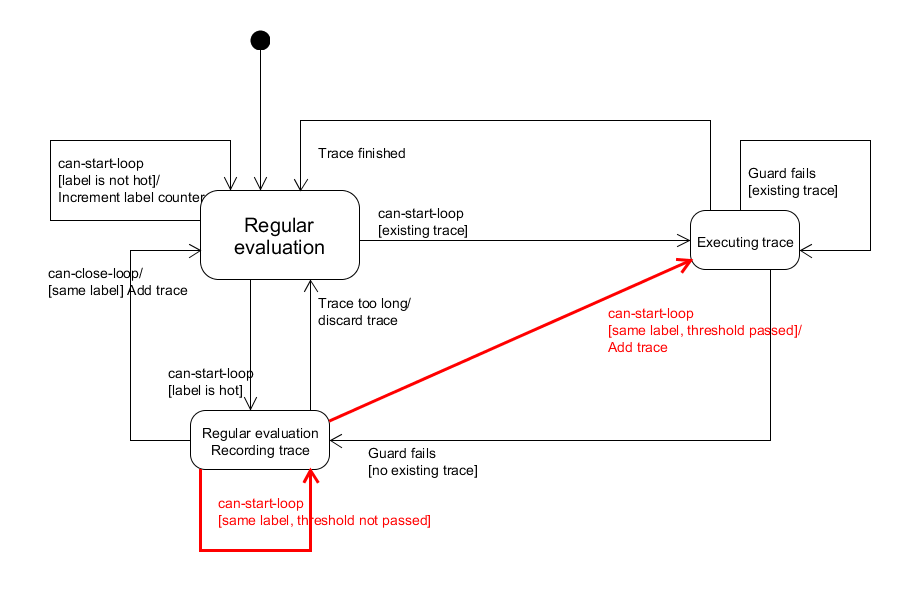
\includegraphics[scale=0.3]{high_level_state_diagram_true_loops.png} 
\end{frame}

\begin{frame}[fragile]{True vs false loops}
True loops = functions which have recursed at least x times
\begin{lstlisting}[basicstyle = \tiny\ttfamily, escapechar = £]
(struct tracer-context (...
                        times-label-encountered-while-tracing
                        ...))

(define (handle-can-start-loop-annotation-reg label debug-info state)
  (cond ((is-tracing-label? tracer-context label)
         (check-stop-tracing-label label state))))
         
(define (check-stop-tracing-label tracer-context label state)
  (define (do-stop-tracing!)
    (stop-tracing! tracer-context #t)
    (let ((new-state (execute-label-trace-with-label label)))
      (step* new-state)))
  (define (do-continue-tracing)
    (execute/trace `(pop-continuation))
    (step* state))
  (inc-times-label-encountered-while-tracing!)
  (if (times-label-encountered-greater-than-threshold?)
      (do-stop-tracing!)
      (do-continue-tracing)))
\end{lstlisting}
\end{frame}

\begin{frame}[fragile]{True vs false loops}
True loops = functions which have recursed at least x times
\begin{lstlisting}[basicstyle = \scriptsize\ttfamily, escapechar = £]
(struct label-trace trace-node ((loops? #:mutable)))
  
(define (handle-can-start-loop-annotation label debug-info state)
  (cond ((label-trace-exists? label)
         (let ((label-trace (get-label-trace label)))
           (if (or (not (is-tracing?)) (label-trace-loops? label-trace))
               ; Record and jump to existing trace
               (let ((new-state (execute-label-trace-with-label label)))
                 (step* new-state))
               ; Ignore existing trace, inline
               (continue-with-state))))
\end{lstlisting}
\end{frame}

\begin{frame}
\centering
\Huge{Fin!}
\end{frame}

\end{document}
